\subsection{\textbf{引言:我们是如何从代码到机器人控制的}}
通过之前的学习,相信大家已经对如何再CMake的帮助下使用C++编写代码有了一定的了解。
之后你们会学习一些针对特殊需求的库,比如OpenCV、cuda等。他们能解决一些特定的问题,比如视觉处理
和模型运行等。

在此之前,你们需要学会如何把将要学的这些内容连接起来。比如,机器人的相机、传感器、MCU发来的信息会不断地
想你发送信息,我们需要一种“系统”能够从容地处理这些信息,对这些信息进行运算再发送出去。
这个“系统”其实就是操作系统(OS, Operating System)。对于个人计算机,我们使用的是Windows、Linux、Mac OS等,
他们帮我们进行了很多底层的工作,比如处理硬件、网络、驱动程序等。
而对于机器人来说,我们使用的是\textbf{ROS}(Robot Operating System),它帮助我们管理多个信息来源和不同信息,同时负责不同模块之间的通信。
这样一来,我们就不必要关注多个线程之间的同步、死锁等问题,只需要专注于业务逻辑的实现。
可以理解为如果不使用ROS2,我们需要自己使用C++的多线程库编写一个复杂的多线程系统,而ROS2可以替代你们上一章学的C++多线程,因为一个复多线程系统的编写
往往setTimeOut、wait等操作非常复杂,而ROS2使用DDS(Data Distribution Service)来实现通信,它已经帮我们处理了很多底层的细节。
\subsubsection{ROS2的版本}
和Linux与Ubuntu的关系类似,ROS2也有不同的版本或者说分支,比如ROS2 Foxy、ROS2 Eloquent等。
现在,我们队伍中主流使用的版本是\textbf{ROS2 Humble Hawksbill}。
\begin{figure}
    \centering
    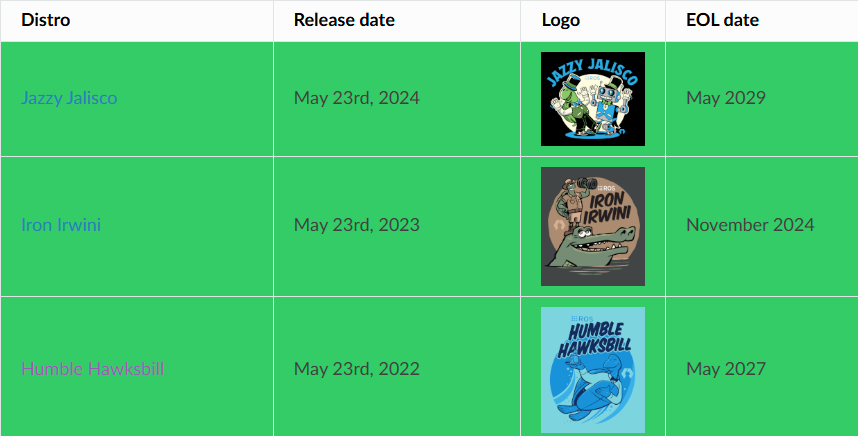
\includegraphics[width=0.8\textwidth]{Chapter4/img/ros2_logo.png}
    \caption{ROS2的最新版本跟新情况}
    \label{fig:ros2_logo}
\end{figure}

\subsubsection{ROS2的安装}

首先,我们需要安装ROS2的Humble Hawksbill 版本。
\begin{tbash}
    wget http://fishros.com/install -O fishros && . fishros
\end{tbash}
这条命令会帮你下载并运行一个脚本,根据它的引导选择下载ROS humble即可。
大概的输出为:
\begin{tbash}
    some output should be here...
\end{tbash}
这是一个非常好用的网站,江湖人称鱼香ROS。

这个命令在配置一个白板的Ubuntu系统时一般第一个运行,它会引导你更换系统源、安装必要的依赖包、配置环境变量等(甚至是下载QQ和微信)
这就减少了去官网上一个个寻找ubuntu版本的麻烦。

\subsection{ROS2架构}
\subsubsection{ROS2的系统架构}
ROS2的系统架构如下图所示:
\begin{figure}[h]
    \centering
    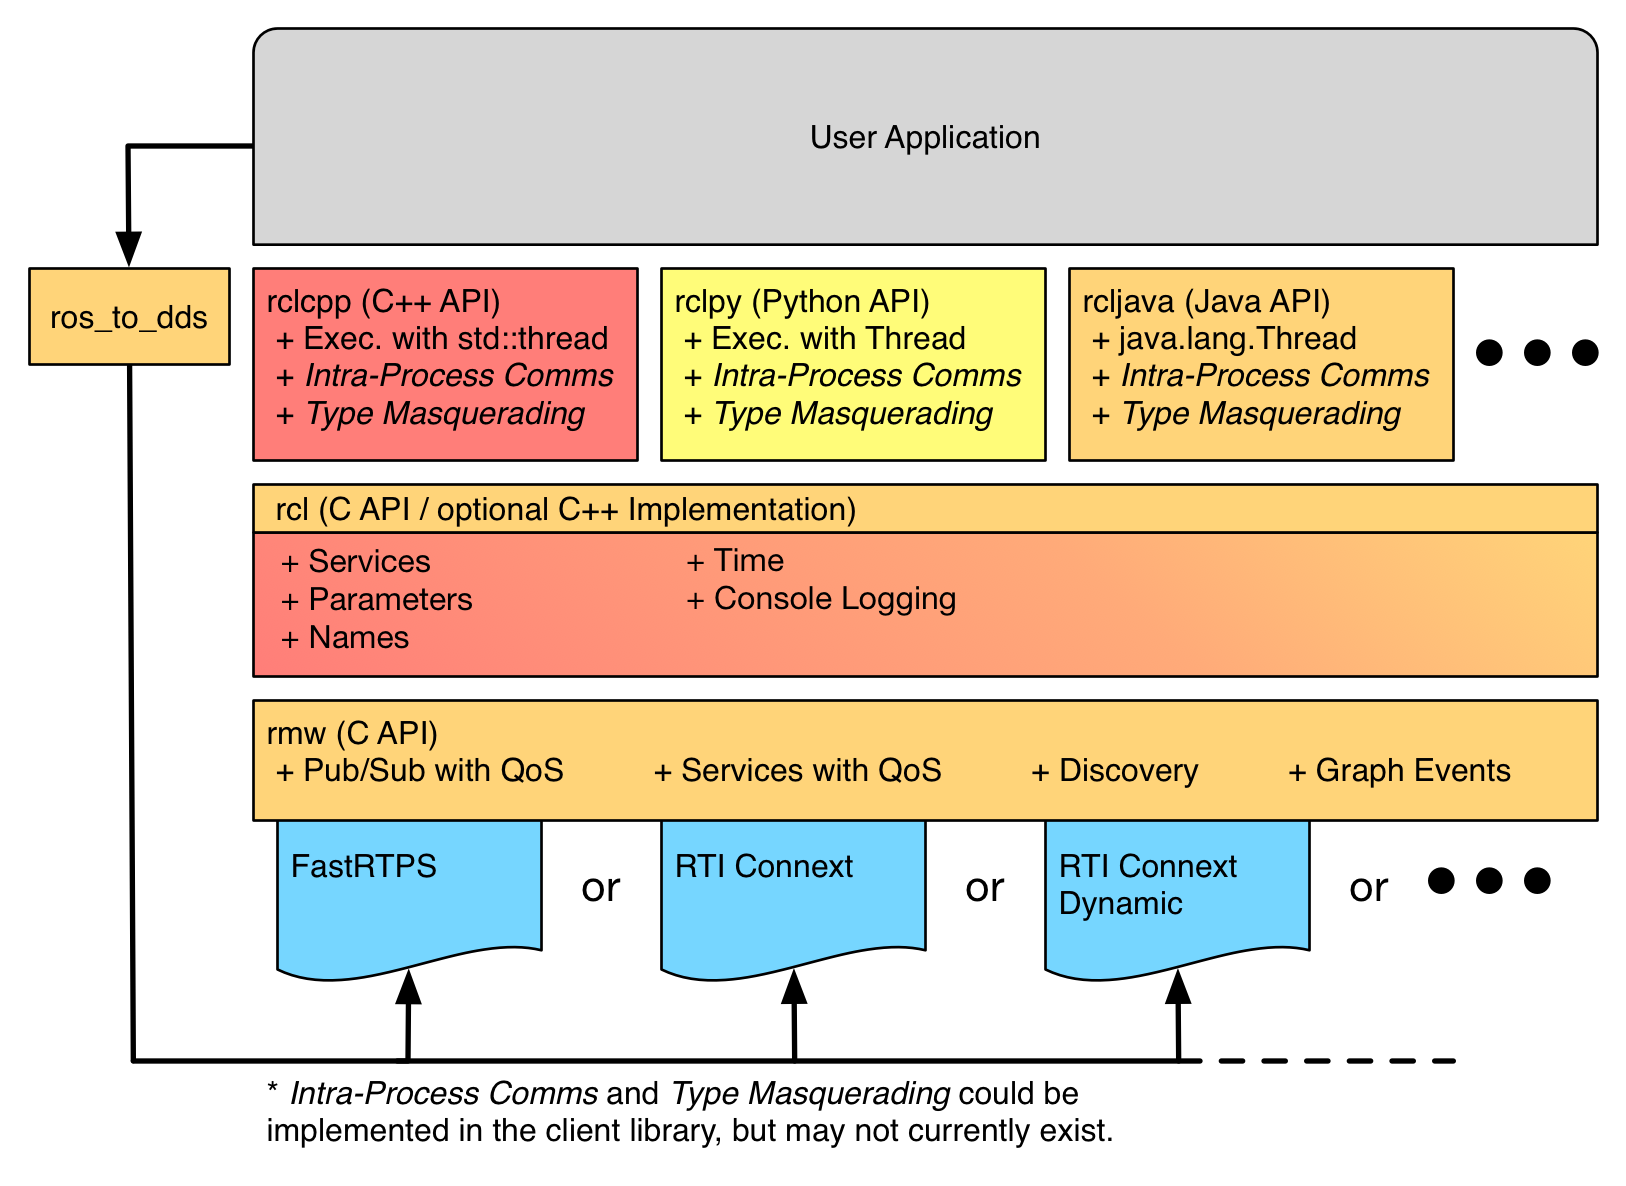
\includegraphics[width=0.8\textwidth]{Chapter4/img/ros2_arch.png}
    \caption{ROS2架构}
    \label{fig:ros2_arch}
    虽然你可能现在看不懂这个图,但不妨等学完之后再回过头来看看。
\end{figure}
一些需要听说过的属于的翻译:
\begin{itemize}
    \item \textbf{rclcpp}: ROS Client Library for C++,它是ROS2的C++客户端库,负责ROS2节点的创建、通信、生命周期管理等,我们使用的主要是这个库。
    \item \textbf{rmw}: ROS Middleware,它是ROS2的中间件,负责底层通信的实现。
    \item \textbf{Qos}: Quality of Service,它是ROS2的通信质量保证机制,用来控制通信的延迟、带宽等。
    \item \textbf{DDS}: Data Distribution Service,它是ROS2的分布式数据服务,用来实现ROS2节点之间的通信。
\end{itemize}
\subsubsection{ROS2的节点与组件}
\textbf{ROS2的基本思想是分布式的、模块化的。}

ROS2的节点是ROS2系统的基本单元,它可以包含多个ROS2组件。

我们可以用这个图来直观地理解ROS2的\textbf{节点}:
\begin{figure}[h]
    \centering
    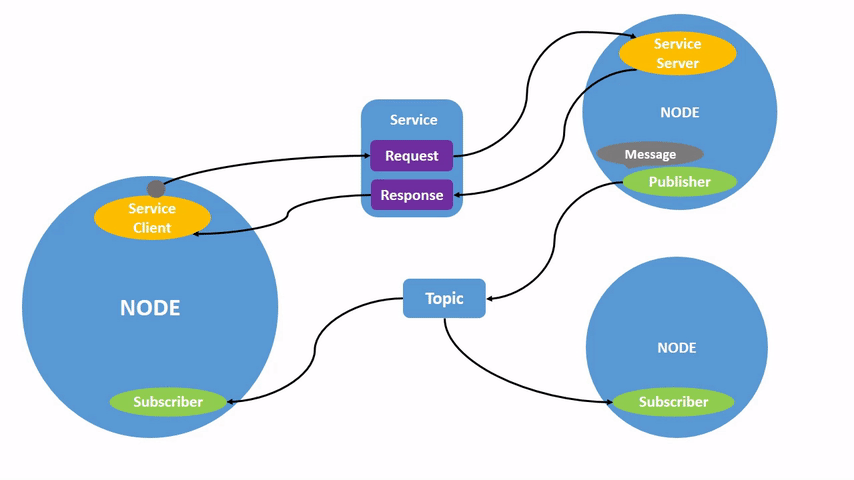
\includegraphics[width=0.8\textwidth]{Chapter4/img/ros2_node.png}
    \caption{ROS2节点与组件}
    \label{fig:ros2_node}
\end{figure}
这是一个动图,你可以去\underline{\href{https://docs.ros.org/en/humble/_images/Nodes-TopicandService.gif}{这里}}播放看看。

这个图直观的反映了ROS2的模块化是依靠\textbf{节点}完成的,节点的职责可以是接收某个传感器的信息(比如相机),也可以是对数据进行处理的流程(比如对相机的图像进行滤波),也可以是提供服务(比如反馈相机的参数信息)
当然这些功能也可以在一个节点中完成。同时可以注意到,节点之间的信息交流是依靠组件(Component)来实现的,一般来说一个节点的运行入口函数也是某个组件的回调函数。


对于我们实际上手操作的情况下,我们更感知的操作方式有两种。
一是使用CLI tools(command-line interface),二是使用Client Libraries。
我们一般使用CLI tools来创建、运行、调试节点,而Client Libraries则用于编写节点的逻辑。

\subsection{ROS2的节点}
ROS2的节点是ROS2系统的基本单元,它可以包含多个ROS2组件,比如发布者(Publisher)、订阅者(Subscriber)、服务(Service)、客户端(Client)等。
下面我们先从什么是节点开始介绍。

\subsection{ROS2}

https://design.ros2.org/articles/roslaunch.html